\documentclass[10pt]{article}

\usepackage[UTF8,fontset=none]{ctex}
\setCJKmainfont[AutoFakeBold=2.5]{Songti SC}
\setCJKsansfont[AutoFakeBold=2.5]{Hiragino Sans GB}
\setCJKmonofont{Songti SC}
\usepackage[a4paper,margin=1.8cm,top=1.6cm,bottom=1.8cm]{geometry}
\usepackage{amsmath,amssymb}
\usepackage{graphicx}
\usepackage{booktabs}
\usepackage{array}
\usepackage{tabularx}
\usepackage{colortbl}
\usepackage{url}
\usepackage{multirow}
\usepackage{xcolor}
\usepackage{enumitem}
\usepackage{listings}
\usepackage{placeins}
\usepackage{float}
\usepackage{tikz}
\usepackage[numbers,sort&compress]{natbib}
\usepackage[colorlinks=true,linkcolor=black,citecolor=black,urlcolor=blue]{hyperref}

\newcolumntype{L}[1]{>{\raggedright\arraybackslash}p{#1}}
\newcolumntype{Y}{>{\raggedright\arraybackslash}X}
\newcommand{\rowtint}{\rowcolor{black!5}}
\newcommand{\thead}[1]{\textbf{#1}}
\newcommand{\medrange}[2]{\mbox{$#1\,{\scriptstyle[#2]}$}}

\setlength{\labelsep}{4pt}
\newlength{\listlabelwidth}
\newlength{\listleftmargin}
\setlength{\listlabelwidth}{6.5pt}
\setlength{\listleftmargin}{\parindent}
\addtolength{\listleftmargin}{2\labelsep}
\addtolength{\listleftmargin}{\listlabelwidth}
\setlist{leftmargin=\listleftmargin,labelsep=\labelsep,listparindent=0pt,
  topsep=\smallskipamount,partopsep=0pt,parsep=0pt,itemsep=2pt}
\setlist[itemize]{align=right,
  labelindent=0pt,labelwidth=\dimexpr\listleftmargin-\labelsep\relax}
\setlist[enumerate]{align=right,
  labelindent=0pt,labelwidth=\dimexpr\listleftmargin-\labelsep\relax}
\setlist[description]{font=\upshape\bfseries,labelwidth=\listlabelwidth,
  labelindent=\dimexpr\listleftmargin-\labelsep-\listlabelwidth\relax}
\setlength{\emergencystretch}{3em}
\renewcommand{\baselinestretch}{1.08}

\definecolor{cakeCodeBlue}{RGB}{34,82,145}
\definecolor{cakeCodeTeal}{RGB}{20,112,112}
\definecolor{cakeCodeString}{RGB}{154,83,20}
\definecolor{cakeCodeAccent}{RGB}{112,48,140}
\lstdefinestyle{cake}{
  language=Python,
  basicstyle=\ttfamily\scriptsize,
  keywordstyle=\color{cakeCodeBlue}\bfseries,
  keywordstyle=[2]\color{black},
  keywordstyle=[3]\color{cakeCodeTeal},
  commentstyle=\color{black!55},
  stringstyle=\color{cakeCodeString},
  morekeywords=[3]{role,pipeline,barrier,smem,tmem,view,tma_load,mma,wait,
    fence_proxy,range},
  deletekeywords=[2]{range},
  literate={@cake.schedule}{{{\color{cakeCodeAccent}\bfseries @cake.schedule}}}{14},
  backgroundcolor=\color{black!2},
  columns=fullflexible,
  keepspaces=true,
  showstringspaces=false,
  numbers=left,
  numberstyle=\tiny\color{black!55},
  numbersep=6pt,
  frame=tb,
  framerule=0.45pt,
  rulecolor=\color{black!35},
  xleftmargin=1.4em,
  framexleftmargin=1.2em,
  framexrightmargin=0.3em,
  framesep=4pt,
  aboveskip=0.6\baselineskip,
  belowskip=0.4\baselineskip,
  captionpos=b
}
\lstset{style=cake}

\newcommand{\cake}{\textsc{Cake}}
\newcommand{\cakeir}{\textsc{Cake IR}}
\newcommand{\flashinferpr}[1]{%
  FlashInfer PR~\##1%
  \footnote{\href{https://github.com/flashinfer-ai/flashinfer/pull/#1}%
    {github.com/flashinfer-ai/flashinfer/pull/#1}}%
}

\title{\textbf{CAKE}：面向前沿内核演进的编译器--智能体协同设计}
\author{%
Zihao Ye\textsuperscript{1}\thanks{同等贡献。}\quad
Yingyi Huang\textsuperscript{1}\footnotemark[1]\quad
Hongyi Jin\textsuperscript{2}\quad
Bohan Hou\textsuperscript{2}\\
Junru Shao\textsuperscript{1}\quad
Zhongming Yu\textsuperscript{1}\quad
Jinqi Chen\textsuperscript{1}\quad
Meghan Cowan\textsuperscript{1}\\
Shiyi Cao\textsuperscript{1}\quad
Shanli Xing\textsuperscript{1}\quad
Hanfeng Chen\textsuperscript{1}\quad
Vinod Grover\textsuperscript{1}\\
Tianqi Chen\textsuperscript{1,2}\quad
Luis Ceze\textsuperscript{1}\\[0.6ex]
\small
\textsuperscript{1}NVIDIA\qquad
\textsuperscript{2}Carnegie Mellon University%
}
\date{}

\begin{document}
\maketitle

\begin{abstract}
GPU 内核智能体与 GPU 编程语言的研究一直各自推进，而两者之间的鸿沟正是专家级内核难以复现之处。内核智能体通常把编译器当作固定的黑盒：它们改进候选生成、变异与排序，但环境只返回编译错误、正确性结果和端到端计时。这些信号既无法指出究竟是哪一项程序决策引发了同步失败、硬件契约违例或流水线停顿，也无法在前沿工作负载暴露能力缺口时随之扩展。与此同时，可供智能体编写的语言也并非为智能体而设计。块级 DSL 隐藏了区分专家内核与仅仅正确的内核所需的线程束专门化、屏障协同和存储层级放置；低级 DSL 虽暴露了这些控制，却要求掌握复杂的布局演算，使智能体更容易犯错且难以定位错误。本文提出 \cake{}，对编译器与智能体进行协同设计。智能体编写 \cakeir{}：一种带类型、显式体现硬件的调度表示。它无需布局代数即可提供细粒度控制，并携带足够信息，使验证器和代价模型能够在编译前推理程序；框架则以局部化的正确性与性能诊断回应。框架本身也是演进对象，因此反复出现的失败会转化为新的验证规则、IR 原语、代价模型校准和可复用优化策略，而非一次性的规避方案。

在 B200 上、实现细节隐藏且严格匹配的 Flash-KMeans 冷启动实验中（每种表示运行三次），在 8000 万 token 预算下，\cakeir{} 最佳候选相对调优后的 FlashML 基线达到中位数 $1.144\times$，而直接编写 CUDA/PTX 为 $0.928\times$。在该冷启动基准之外，智能体生成的 Kimi Delta Attention 相对官方 FlashKDA 取得 $2.05\times$ 的几何平均加速，并通过端到端服务验证。由调度器支持的 KNN 与 KMeans 系列在 400 多种形状上将性能提升 $1.42\times$--$2.12\times$，另有四项内核改动以向上游 PR 的形式提供。\cake{} 面向从 Ampere 到 Blackwell 的 NVIDIA GPU，并将单一形状的演进与库集成所需的泛化和分派阶段明确分开。
\end{abstract}

\section{引言}
\label{sec:intro}

编码智能体如今已能在自动测量正确性与性能的环境中编写和修订 GPU 程序\cite{ouyang2024kernelbench,liao2025kernelevolve,dong2026kernelblaster,accelopt2025,autocomp2025,cheng2026kernelagent,dai2026cudaagent}。然而，多数系统仍把编程环境视作固定黑盒：智能体提出代码、编译、运行数值测试、测量延迟，再选择下一次修改。这个循环适用于局部调优，但程序崩溃时不会指出违反了哪项安全或硬件条件，单个延迟数字也无法解释究竟哪一项程序决策限制了性能。

专家内核程序员的工作方式不同。他们维持对工作负载的紧凑模型，围绕显式硬件资源推理，并把可复用规则迁移到不同内核之间。编译器其实已拥有将这一过程外显所需的大部分机制：结构化操作词汇、资源模型、合法性检查、静态分析、代价模型和 lowering 规则。\cake{} 所追问的是，如何让智能体直接使用这些机制，以及当前沿工作负载暴露缺口时如何改进它们。

\cake{} 作出三项承诺。第一，智能体编辑带类型的 IR，而不是原始 CUDA，因此代码生成之前就能检查硬件决策。第二，编译器返回局部化的正确性与性能诊断，而不是单一的通过/失败信号，从而让低成本分析在候选消耗 GPU 时间之前完成筛选。第三，框架本身也是演进对象：反复出现的失败会转化为验证规则、校准任务或新原语，并由语料测试把关。\cakeir{} 通过智能体在生产内核语料上自底向上的抽象发现而设计，其准则是必须复现专家内核的物理调度与性能（图~\ref{fig:ir-evolution}；过程详见原文附录）。该框架同样主要由智能体维护，并由人工合并门控把关。

系统支持两种入口，对应内核工作的两种实际来源。它既可以从 FlashInfer 或 CUTLASS 等库中的生产内核出发并继续演进该实现；也可以在没有成熟参考实现的工作负载上，从高层描述或 Triton 实现出发，让智能体在 \cakeir{} 中选择线程束专门化、布局和流水线结构，由编译器验证程序并生成 CUDA。

本文同时报告上述第二种模式和第一种模式下的结果。\cake{} 面向从 Ampere 到 Blackwell 的 NVIDIA GPU，其已验证语料覆盖数十种内核族，包括注意力与线性注意力、稠密/分组/量化 GEMM、MoE 数据流、归一化、量化、Top-$K$、KNN、KMeans 和融合图内核。第~\ref{sec:evaluation} 节评估针对调优基线的重复冷启动演进，报告 Kimi Delta Attention~\cite{kimi_linear2025}、Gated DeltaNet~\cite{gated_deltanet2025} 和稀疏注意力等模型架构上的前沿内核合成，并报告对既有内核族的复现。第~\ref{sec:generalization} 节进一步处理基准数字通常略过的一步：如何把针对单一形状调优的内核转化为服务库可在任意形状下调用、由调度器支持的内核族。

\begin{figure}[!htbp]
  \centering
  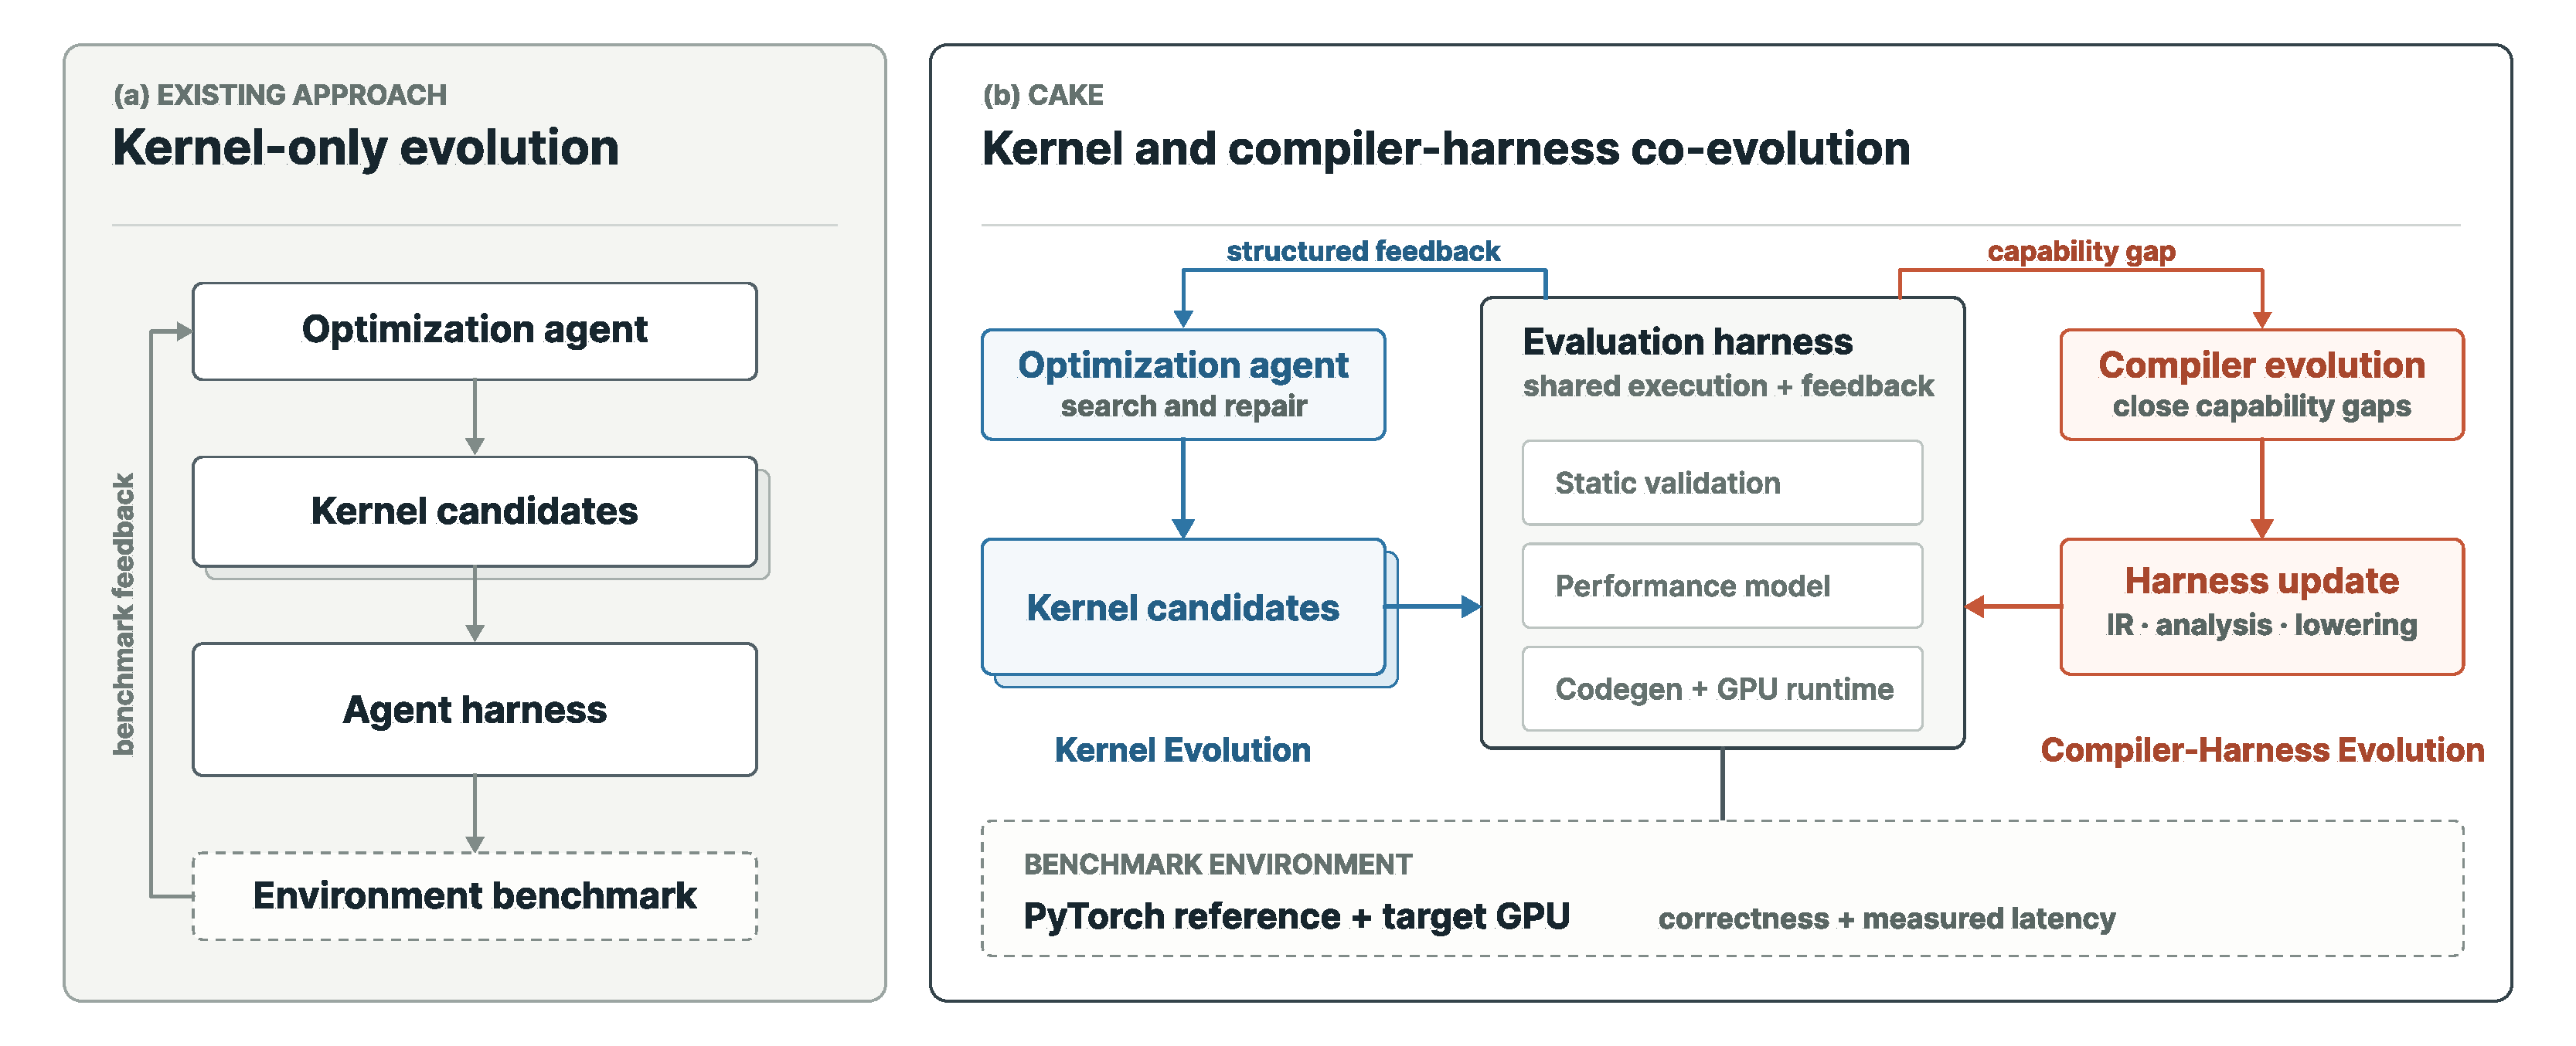
\includegraphics[width=0.99\linewidth]{figures/cake_overview_comparison.pdf}
  \caption{\cake{} 概览。内核演进以结构化编译器证据为输入；编译器演进构成外层循环。}
  \label{fig:overview}
\end{figure}

\FloatBarrier

\section{程序表示}
\label{sec:representation}

\cake{} 将 \cakeir{} 作为面向智能体的程序表示，并生成 CUDA/PTX 以执行程序。结构化分析和性能建模在 \cakeir{} 上运行，常规的 sanitizer 与 profiler 反馈则来自生成的代码。

\subsection{自底向上的 IR 演进}
\label{sec:bottom-up-ir}

\cake{} 并非从预定义的 \cakeir{} 词汇表起步。它的初始材料是生产内核语料与硬件设计原则。智能体从这些内核中识别反复出现的调度模式或缺失能力，修订 IR 及其编译器支持，再移植内核并在修订后的系统上验证。下一个内核族，或验证暴露出的缺口，会再次启动同一循环。这个循环既产生了当前的 IR，也持续扩展它（图~\ref{fig:ir-evolution}；详细过程见原文附录）。

\begin{figure}[!htbp]
  \centering
  \resizebox{\linewidth}{!}{%
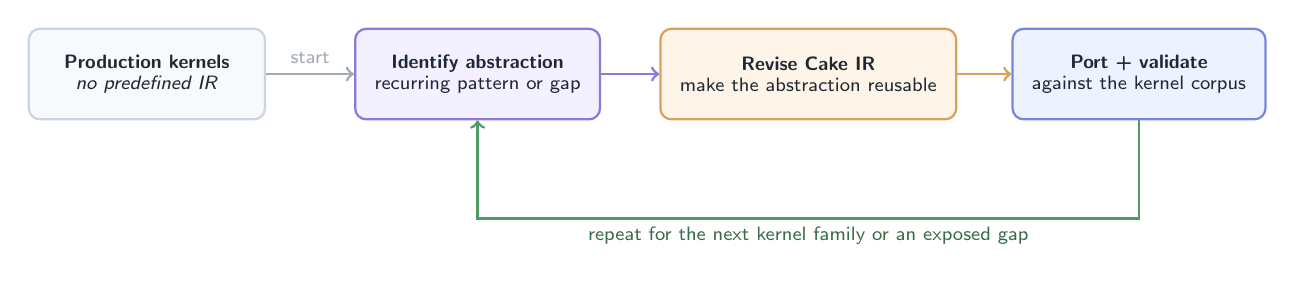
\begin{tikzpicture}[
  font=\sffamily\scriptsize,
  box/.style={rectangle, rounded corners=4pt, draw, line width=0.8pt,
    align=center, inner xsep=7pt, inner ysep=6pt, minimum height=1.15cm},
  flow/.style={->, line width=1.0pt},
  note/.style={font=\sffamily\scriptsize, align=center},
]
\definecolor{irText}{HTML}{1F2933}
\definecolor{irNeutralFill}{HTML}{F7F9FC}
\definecolor{irNeutralBorder}{HTML}{CBD5E1}
\definecolor{irKnowledgeFill}{HTML}{F3F0FF}
\definecolor{irKnowledgeBorder}{HTML}{8B7BD6}
\definecolor{irCandidateFill}{HTML}{FFF4E8}
\definecolor{irCandidateBorder}{HTML}{D9A05B}
\definecolor{irValidationFill}{HTML}{EEF2FF}
\definecolor{irValidationBorder}{HTML}{7687D9}
\definecolor{irSuccessBorder}{HTML}{4F9B65}
\color{irText}

% One external starting point, followed by one repeating three-step loop.
\node[box, fill=irNeutralFill, draw=irNeutralBorder, minimum width=3.0cm]
  (corpus) at (0,0) {\textbf{Production kernels}\\[-1pt]
    \emph{no predefined IR}};
\node[box, fill=irKnowledgeFill, draw=irKnowledgeBorder, minimum width=3.0cm]
  (discover) at (4.2,0) {\textbf{Identify abstraction}\\[-1pt]
    recurring pattern or gap};
\node[box, fill=irCandidateFill, draw=irCandidateBorder, minimum width=3.0cm]
  (revise) at (8.4,0) {\textbf{Revise \cakeir{}}\\[-1pt]
    make the abstraction reusable};
\node[box, fill=irValidationFill, draw=irValidationBorder, minimum width=3.0cm]
  (validate) at (12.6,0) {\textbf{Port + validate}\\[-1pt]
    against the kernel corpus};

\draw[flow, color=irNeutralBorder!80!black]
  (corpus) -- node[note, above] {start} (discover);
\draw[flow, color=irKnowledgeBorder] (discover) -- (revise);
\draw[flow, color=irCandidateBorder] (revise) -- (validate);

% The large return path is the main point of the figure: IR construction never
% terminates at a final box.
\draw[flow, color=irSuccessBorder]
  (validate.south) -- ++(0,-1.25) -| (discover.south);
\node[note, below, color=irSuccessBorder!70!black]
  at (8.4,-1.82) {repeat for the next kernel family or an exposed gap};
\end{tikzpicture}%
}

  \caption{\cakeir{} 从内核而不是固定语言设计中演进。初始语料只进入一次；此后三步循环会针对每个新内核族或能力缺口重复执行。}
  \label{fig:ir-evolution}
\end{figure}

\FloatBarrier

\subsection{\cakeir{} 中的显式机器调度}
\label{sec:cake-ir}

\cakeir{} 记录应当如何驱动机器：哪些线程束承担哪些角色、哪些缓冲区以多深的阶段数进行暂存、哪个屏障控制哪一次交接、哪种指令形式消费哪一个操作数。相应的分工是：调度声明\emph{要做什么}，lowering 推导\emph{如何完成}。屏障地址、相位位、TMEM 偏移、描述符编码和线程束身份都由声明计算得到，而不是由智能体手写。

一个程序组合了显式操作、声明式资源、线程束角色以及网格与流水线配置（图~\ref{fig:ir-example}）。四项性质发挥核心作用。\emph{类型检查词汇}：计算、数据移动、同步、数学和线程束控制采用固定 IR 词汇，而非嵌入式 C 或 PTX。\emph{声明式资源}：内存区域、同步状态和流水线只声明一次，因此 IR 掌握每个缓冲区的形状、数据类型和生命周期。\emph{显式角色}：线程束组均有名称，跨角色交接全部可见，而不是隐含约定。\emph{自动推导元数据}：这些声明的机械性结果由 lowering 生成，无需人工编写。

\begin{figure}[t]
\begin{lstlisting}
@cake.schedule()
def fmha_fwd(lm, Q: LM.tma3d, O: LM.tma2d, seqlen_q: LM.i32):
    # declare resources: named resources, not raw addresses
    pool     = lm.smem(98304)
    smem_q   = pool.view(offset=0, shape=(128,128), dtype=lm.bf16, stage=3)
    tmem_acc = lm.tmem(cols=0, width=128, shape=(128,128), dtype=lm.f32)

    # declare roles: warp groups with assigned work
    load = lm.role(warps=[0])
    mma  = lm.role(warps=[1])
    pipe = lm.pipeline(stages=3)
    q_full = lm.barrier(count=3, prod=[load], cons=[mma],
                        init_count=1, pipeline=pipe)

    with load:
        for stage in lm.range(0, 3):
            smem_q.tma_load(Q, coords=(0,0,stage), stage=stage, barrier=q_full)

    with mma:
        for stage in lm.range(0, 3):
            lm.wait(q_full, stage=stage)
            lm.fence_proxy()
            lm.mma(tmem_acc, smem_q[stage], smem_q[stage], init=(stage == 0))
\end{lstlisting}
\caption{一个 \cakeir{} 调度片段。资源与角色通过声明给出；生产者--消费者交接是显式屏障；地址、相位与线程束身份由 lowering 推导。}
\label{fig:ir-example}
\end{figure}

其收益在于，分析可以在代码生成之前依据显式调度决策进行推理。因此，框架能够把发现绑定到受影响的资源、角色或阶段，而不是只返回后端错误或程序挂起。语言目录、资源模型和设计原则详见原文附录。

\paragraph{布局。}
\cake{} 有意不把布局设为一等抽象。\cakeir{} 不要求智能体操纵布局代数，而是直接在调度中记录存储与访问决策。编译器随后检查生产者与消费者表示是否兼容目标硬件（详见原文附录）。

\subsection{体系结构与 lowering}
\label{sec:arch}

同一套调度语言面向从 Ampere 到 Blackwell 的 NVIDIA GPU，因此“角色--屏障--流水线”调度在结构上可移植，而指令准入与 lowering 仍因目标而异。\cake{} 会精确映射所连接的 GPU；对于不支持的目标，它会明确报告，而不会静默替换为其他体系结构；只有目标专用校准可用时才会输出性能估计。详细设备矩阵和后端说明见原文附录。

\section{编译器框架}
\label{sec:harness}

该框架是围绕 \cakeir{} 构建、面向智能体的环境。人类给出预期分析的高层描述，智能体则在验证约束下实现、维护和细化这些分析。在内核演进期间，低成本分析会在候选进入昂贵的 GPU 运行之前完成排序与筛选。

\subsection{分析与验证}
\label{sec:analysis}

\paragraph{程序安全与硬件一致性。}
编译之前，框架会检查带类型调度中大类的同步、内存安全、数据流、资源、指令和数据表示违例。这些检查会拒绝许多在数学上看似合理、却不符合目标执行模型的候选。每项发现都指出受影响的程序区域与被违反的契约类别，从而通过稳定的分析接口为智能体提供可操作的修复目标。

\paragraph{数值正确性。}
对于每个工作负载，我们在不同形状和输入分布上比较内核输出与参考输出。最终验收要求在相应目标框架中进行端到端评估。

\paragraph{性能建模。}
经校准的代价模型估计候选性能，并返回高层瓶颈归因和优化指导。模型用于候选排序与筛选；设备实测和性能分析仍是最终事实依据。

表~\ref{tab:analysis-categories} 按外部可见功能而非单个 pass 或具体实现汇总该套件。关键接口是其契约：阻断式检查以局部化理由拒绝候选，报告描述可能的性能限制，提示则给出非阻断式优化建议。

\begin{table}[H]
  \caption{\cake{} 框架向外暴露的分析与验证类别。类别描述用户可见行为，而非内部 pass。}
  \label{tab:analysis-categories}
  \centering
  \footnotesize
  \setlength{\tabcolsep}{4pt}
  \renewcommand{\arraystretch}{1.06}
  \begin{tabularx}{\linewidth}{@{}L{3.3cm}L{2.5cm}Y@{}}
    \toprule
    \thead{类别} & \thead{处置方式} & \thead{目的} \\
    \midrule
    \rowtint
    程序安全 & 编译前门控 & 识别同步、顺序和内存使用风险 \\
    硬件一致性 & 编译前门控 & 强制执行受支持的资源、指令和体系结构契约 \\
    \rowtint
    数据一致性 & 编译前门控 & 检查数据流及生产者--消费者表示兼容性 \\
    调度语义 & 编译前门控 & 检查声明式调度的结构不变量 \\
    \rowtint
    数值验证 & 执行门控 & 将编译后输出与权威外部参考进行比较 \\
    性能分析 & 报告 & 估计代价并识别大类瓶颈 \\
    \rowtint
    优化指导 & 提示 & 在不阻断编译的情况下建议有潜力的修订 \\
    \bottomrule
  \end{tabularx}
\end{table}

\subsection{编译器演进}
\label{sec:compiler-evolution}

\cake{} 让编译器与内核共同演进。内核候选、验证结果、基准测试和失败报告共同构成提出并验证编译器改动的证据。

编译器演进沿两条互补路径进行（图~\ref{fig:orchestration}）。第一条路径中，智能体检查生产内核与硬件文档，寻找缺失的 Blackwell 模式，例如新指令形式、资源类型、描述符变体和同步惯用法，并据此提出编译器改动。每项提案在实现前都会依据 \cakeir{} 的设计原则进行检查，其中包括性能透明性和验证友好性。第二条路径中，智能体利用失败候选的反馈，例如 sanitizer 报告、失败用例、正确性不匹配和调试日志，将反复出现或代价高昂的失败模式提炼为新分析：不透明的运行时崩溃会变成验证器规则，反复出现的非法 lowering 模式会变成静态检查，系统性误判则会变成校准目标。

两条路径相互耦合。新原语向编译器暴露更多硬件事实，使更强的分析成为可能；新分析反过来约束未来原语的设计空间。编译器改动必须通过整个内核语料的测试门控，因为原语及其分析必须一同演进：只有语法而缺乏效果与合法性规则会降低 IR 的可分析性，而未经语料验证的新验证器规则则可能拒绝合法内核。

\begin{figure}[t]
  \centering
  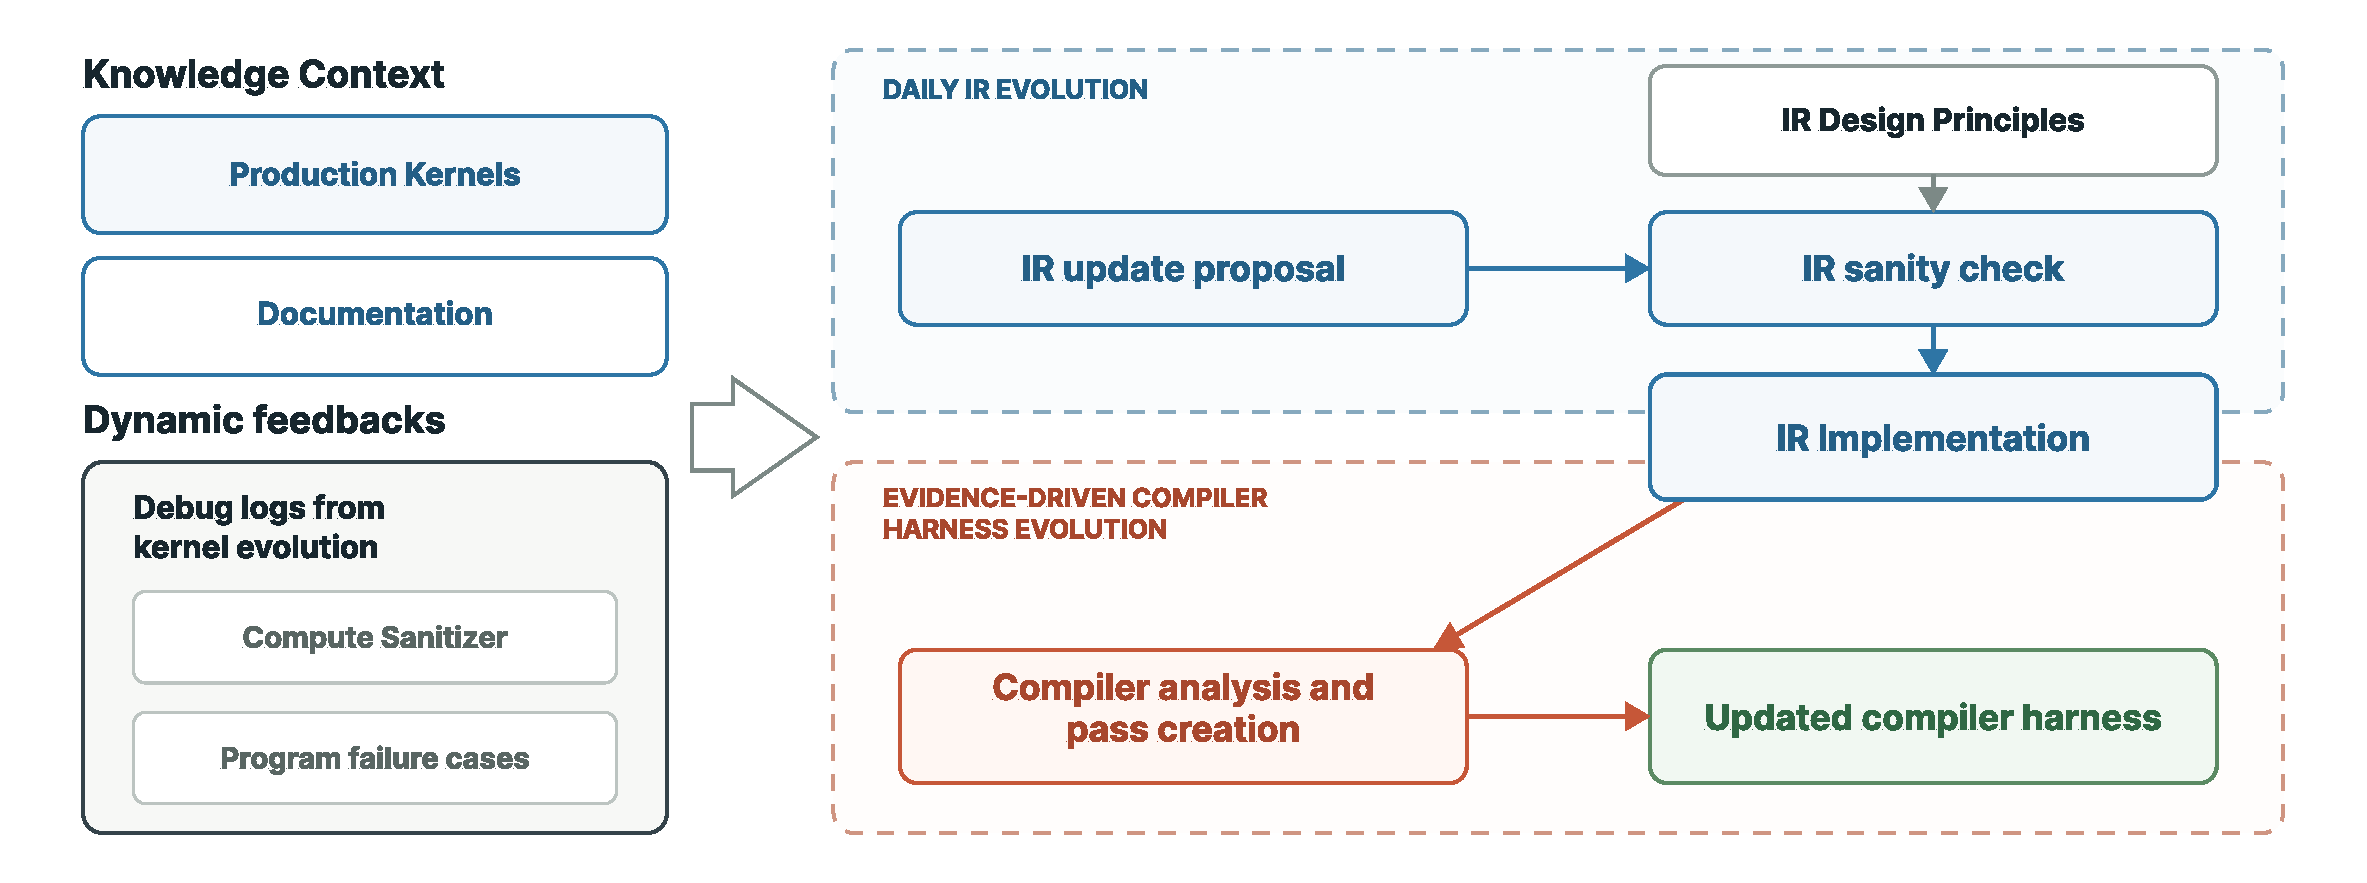
\includegraphics[width=0.9\linewidth]{figures/compiler_harness.pdf}
  \caption{证据驱动的编译器演进。语料与运行时证据共同驱动经过验证的编译器改动。}
  \label{fig:orchestration}
\end{figure}

\section{智能体工作流}
\label{sec:workflow}

外部工作负载契约是稳定的权威依据。一次运行包含四个阶段：生成结构不同的 \cakeir{} 候选；在消耗 GPU 时间前，利用 IR 构造检查、验证器硬门控和代价模型排序筛选候选；针对外部预言机评估幸存候选，并收集基准测试与 profiler 证据；最后根据诊断，将所得证据路由到候选、验证器、代价模型或 IR 词汇。工作负载契约固定形状、预言机、容差、硬件和允许访问的参考，而保留的结果使决策可审计，也使反复出现的发现可复用。

所有报告的智能体任务均使用 GPT-5.6-sol~\cite{openai2026gpt56}，推理强度为 \texttt{xhigh}。固定模型与智能体脚手架，使第~\ref{sec:evaluation} 节的比较可归因于环境，而不是模型能力差异。

\section{评测}
\label{sec:evaluation}

评测回答三个问题：编译器框架能否推动重复冷启动演进超过调优后的基线；\cake{} 能否在没有低级实现参考的情况下合成前沿内核；以及它能否对照最先进基线复现专家内核。

\paragraph{实验协议。}
所有测量均在 B200 上使用 GPU 端正确性检查与 CUPTI 计时，并在每个计时样本前清空 L2 缓存。每个报告的候选都会在列出的形状上编译、检查正确性并运行基准测试。

重复冷启动实验固定编码智能体及其脚手架、模型和推理强度、任务描述、正确性预言机、基准测试框架以及单一目标形状。Flash-KMeans 实验使用隔离的 B200 冷启动环境；该环境提供任务规范、正确性预言机和基准接口，但隐藏目标的低级实现。处理组编写带类型的 \cakeir{}，对照组则直接编写 CUDA C++ 和内联 PTX。我们报告供应商 token 消耗量与主动演进时间。表~\ref{tab:kmeans-cleanstart} 汇总了每个实验组在 8000 万 token 预算下的三次匹配运行，图~\ref{fig:clean-start-evolution-token-performance} 展示其符合条件的性能检查点。汇总项采用中位数 $[\mathrm{min},\mathrm{max}]$；详细停止条件与计时核算保存在配套制品中。

\paragraph{参考访问策略。}
允许访问哪些参考取决于所回答的问题。在冷启动与前沿内核合成中，智能体可以检查数学规范、评测契约、正确性预言机和高层代码，但不得检查 CUDA、PTX、SASS 或同等生成源码等低级目标实现。这些参考已编码了实验要求智能体自行发现的调度决策。外部实现仍可作为黑盒性能基线由基准框架执行，但其内部细节对智能体不可见。在已知内核复现中，智能体可以查看参考实现。Flash-KMeans 的限制在隔离冷启动环境中执行，并在事后审计。直接 CUDA/PTX 组改变的是所编写的表示，而不是参考策略：该组可以编写低级代码，但不能检查已有的目标实现。

\paragraph{Flash-KMeans 冷启动工作负载。}
为测试从实现隐藏的冷启动出发能否复现结果，我们使用 Flash-KMeans~\cite{Yangetal2026FlashKMeans}。这是一个精确 $k$-means 工作负载，动机来自 Sparse VideoGen2 中的语义感知 token 置换~\cite{Yangetal2025SparseVideoGen2}。一次 Lloyd 迭代主要由两个 BF16 内核主导，二者占端到端时间的 95\% 以上：\texttt{assign} 计算每个 token 到全部 $K$ 个质心的平方欧氏距离并返回 arg-min；\texttt{centroid\_update} 则把每个簇内的 token 归约为逐簇求和与计数。两者具有不同特征：\texttt{assign} 是计算受限的 BF16 GEMM 加归约内核，而 \texttt{centroid\_update} 对带宽和原子操作争用敏感。我们聚焦 \texttt{assign}；其在 $B{=}32$、$N{=}65{,}536$、$K{=}1024$、$D{=}128$ 下使用 BF16 输入与 FP32 累加器，覆盖 Tensor Core 流水线和标量尾处理。所有运行采用相同模型、预言机与基准测试。性能归一化到经过调优的 FlashML KMeans Triton 实现，该基线实测为 $0.938$\,ms。

\begin{table}[H]
  \caption{B200 上匹配的三次 Flash-KMeans 冷启动比较。}
  \label{tab:kmeans-cleanstart}
  \centering
  \footnotesize
  \setlength{\tabcolsep}{5pt}
  \renewcommand{\arraystretch}{1.12}
  \begin{tabular}{@{}lccc@{}}
    \toprule
    \thead{表示} &
      \thead{\shortstack{截至 80M\\达到平台}} &
      \thead{\shortstack{主动演进\\时间（小时）}} &
      \thead{\shortstack{80M 时\\最佳性能}} \\
    \midrule
      \cakeir{}
      & 3/3
      & \medrange{1.89}{1.02,2.33}
      & \medrange{1.144}{1.041,1.205} \\
      直接 CUDA/PTX
      & 0/3
      & \medrange{3.73}{3.59,4.34}
      & \medrange{0.928}{0.852,1.151} \\
    \bottomrule
  \end{tabular}
\end{table}

\paragraph{演进轨迹。}
图~\ref{fig:clean-start-evolution-token-performance} 展示性能增益何时出现，从而补充表~\ref{tab:kmeans-cleanstart} 中的终点汇总。\cakeir{} 组的均值在 5500 万 token 时越过调优后的 FlashML 基线，并继续改善；直接 CUDA/PTX 组的均值到 8000 万 token 截止点仍低于基线。

\begin{figure}[t]
  \centering
  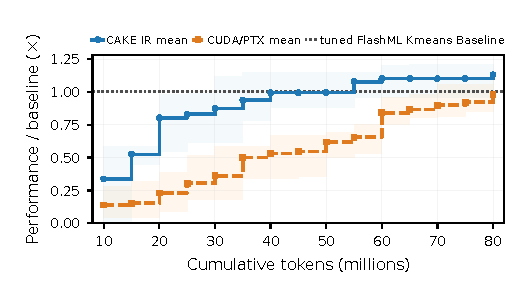
\includegraphics{figures/flash_kmeans_cleanstart_three_run.pdf}
  \caption{B200 上 Flash-KMeans 固定形状冷启动的达成情况。从 10M 到 80M，每隔 5M token 的预算点，每次运行都贡献截至该点最佳的已验证加速比。曲线表示三次运行均值，阴影带表示运行间最小值--最大值，水平线表示调优后的 FlashML K-means 基线。}
  \label{fig:clean-start-evolution-token-performance}
\end{figure}

在匹配运行中，\cakeir{} 在 8000 万 token 前有 3/3 次达到预先规定的平台标准，而直接 CUDA/PTX 为 0/3。相对调优后的 FlashML 基线，前者的最佳达成中位数为 $1.144\times$，后者为 $0.928\times$；主动演进时间中位数分别为 1.89 小时与 3.73 小时。

\FloatBarrier
\subsection{前沿内核合成}
\label{sec:eval-frontier}

这里所说的“前沿”具有操作性定义：智能体必须在不检查低级目标实现的情况下发现物理调度。已有实现仍可作为黑盒评测基线。协同演进的 IR 最有可能在这一模式中发挥作用，因为搜索无法锚定到已知优良设计；与此同时，这一模式也最能暴露框架的不足，因为能力缺失会直接表现为智能体完全无法表达某种调度。

\paragraph{新兴模型架构。}
Kimi Delta Attention（KDA）是最清晰的案例。官方 FlashKDA 仅作为黑盒计时基线使用，其源码与生成代码均不提供给智能体。一个兼容 FlashKDA 的 prefill 实现覆盖固定输入、打包变长输入和尾部输入，在六个 B200 BF16 形状上相对该基线达到 $2.05\times$ 的几何平均加速。它在验证契约上逐位正确，并已在 SGLang 下的端到端 Kimi-K3 服务中得到验证。生成的 CUDA 可见于 \flashinferpr{4262}，因此下游用户无需依赖 \cake{}。独立的 decode 路径在 30 个公共 API 形状上相对上游 FlashInfer 达到 $1.14\times$ 的几何平均性能（\flashinferpr{4279}）。不同于带尾处理的 GEMM，KDA 包含必须跨块保持存活的循环状态，因而能有效检验调度表示。相应的两阶段源会话轨迹见原文附录。

对比 FlashInfer，Gated DeltaNet 的 prefill 与 speculative-decode 路径在保留模型循环状态的同时提升了性能。MiniMax 稀疏注意力进一步表明，同一表示能够支持 prefill 与 decode 两种路径上的稀疏注意力族。这些都是分派族而不是单一内核：不同物理调度以独立 \cakeir{} 程序的形式保留在同一逻辑入口之后。

\paragraph{参考引导的生产演进。}
TinyGEMM 为上述冷启动前沿实验提供了互补的生产案例。智能体从 FlashInfer 中源自 TensorRT-LLM 的小 $M$ BF16 内核出发，生成了浅层和深层流水线组成的自适应内核族，其中包括 PDL 变体和小于 8 的批大小。\flashinferpr{4274} 报告在 35 个标准形状以及更广泛回归测试上，内核时间的几何平均下降 18--23\%。在 B200 与 GB300 上，GPT-OSS-20B 和 GPT-OSS-120B 的贪心解码保持逐位一致；另一次独立的 SGLang GPT-OSS-120B 实验报告，在 TP1、并发度 128 时输出吞吐量最高提升 7.6\%，而 TP4 上的差异处于测量噪声范围内。先前的四形状搜索与针对小形状的后续优化详见原文附录。

\paragraph{通信密集型巨型内核演进。}
Alpha-MoE 的原始实现~\cite{alpha_moe2025} 面向 Hopper。\cake{} 智能体从该实现出发，成功将其 W8A8 融合 MoE 巨型内核重写到 Blackwell。所得实现检验演进中的编译器能否表达围绕 Tensor Core 计算的数据交换，而不只是计算本身。它把路由 gather、两次投影、激活、重新量化和按路由权重累加输出融合到一个设备程序中。

相对于 FlashInfer 中源自 TensorRT-LLM 的预路由 API，它在 $N{=}256$ 与 $N{=}512$ 时的 API 级端到端加速比分别为 $6.204\times$ 和 $4.025\times$。以 GPU span 重新测量后，加速比分别为 $1.215\times$ 与 $1.170\times$，从而单独体现有效 GPU 执行上的改进。更大的 API 级增益还来自启动/调度融合所减少的调度空隙，以及更简单的工作空间处理：参考实现启动五项 GPU 活动，而 Alpha-MoE 只使用一次输出重置与一个巨型内核。对应的 FlashInfer 贡献是 \flashinferpr{4287}。归一化重写轨迹见原文附录；其分母是首个正确的 \cake{} 检查点，而不是 TensorRT-LLM。

\FloatBarrier
\subsection{已知内核复现}
\label{sec:eval-known}

为了验证输出是否达到生产质量，我们还针对现代 LLM 执行路径上具有最先进基线的已知算子族进行实验：注意力前向/反向与 decode、低精度 GEMM，以及 MQA/MLA logits 与 decode 内核。参考实现来自 TensorRT-LLM~\cite{tensorrtllm}、CUTLASS~\cite{cutlass}、DeepGEMM~\cite{deepgemm2025}、FlashAttention-4~\cite{zadouri2026flashattention4algorithmkernelpipelining} 和 FlashInfer~\cite{flashinfer}。这些案例检验的问题不同于前沿内核合成：已有专家结构时，协同演进的框架能否帮助智能体在保持正确性的同时追平或超过高度优化的内核？比较设置本身是固定的，包括内核集合、每种变体列出的参考以及评测形状，因此重跑只会改变数值，不会改变待检验的主张。完整的逐内核矩阵、测量形状、相对性能和经审计的实现规模均见原文附录。

在当前测量的 11 组固定比较中，10 组达到或超过所列参考，剩余一组达到参考性能的 96.5\%。最强结果是两个 MQA indexer，均约为 $1.27\times$。所有比较都通过各自内核特定的正确性门控，并采用 CUPTI GPU span 的中位数。

理解这些结果时需考虑两个因素。低于参考的变体通常反映编译器集成成熟度，而不是采用了不同算法目标：当内核所需特性仍在集成到编译器和代码生成器中时，提交的制品采用当前最接近的受支持策略。相反，表现最强的 indexer 并非对参考内核的忠实转写。在移植过程中，智能体探索了原实现中没有的优化，并保留通过正确性与基准测试的变体，因此高于参考的结果不仅来自转写保真度，也来自搜索。

代码行数列仅作描述，不能作为跨语言的生产力或可读性指标。表中每个 \cakeir{} 实现都短于经审计的参考设备核心，但语言和统计范围不同。该比较只能说明，受测硬件调度可以在 \cakeir{} 中得到紧凑表示，同时保留分析与 lowering 所需的决策。

\subsection{内核组合}
\label{sec:eval-portfolio}

前述评测没有充分反映该框架目前所支撑的广度。经过验证的语料包含 400 多个静态与编译用例，以及横跨约 28 个内核族的 399 个 GPU 正确性用例，覆盖注意力、稠密与稀疏 GEMM、MoE、量化、归一化、状态空间模型、KNN 和 KMeans。它还包含从 Ampere 到 Blackwell 的体系结构专用路径。

除第~\ref{sec:eval-frontier} 节的前沿内核之外，这套语料的另一突出性质是组合能力。由于角色、屏障与缓冲区都通过声明而不是隐含约定给出，通常需要拆成多个内核的调度可以表达为一个设备程序。BatchAttention 组合 decode 与 prefill 工作，Alpha-MoE 和 mega-MoE 内核族则在不物化中间结果的情况下融合路由、专家计算和输出累加。语料还包含 100 多个 TensorRT-LLM 移植，覆盖注意力、MLA decode 与 MoE 内核。原本面向 Hopper 的 Alpha-MoE W8A8 内核由 \cake{} 智能体重写到 Blackwell，说明即使目标指令发生变化，调度结构仍可保留。

四项上游改动分别涵盖 KDA prefill、KDA decode、TinyGEMM2 和 Alpha-MoE。

\section{从单一调优形状到程序库}
\label{sec:generalization}

到目前为止，所有工作都在优化一个形状，而程序库必须接受调用者传入的任意形状。弥合这一鸿沟并不是简单地在更多形状上运行内层循环；它是一个具有不同目标、排序信号和失败模式的独立阶段，\cake{} 也据此将其单独处理。

\paragraph{分离目标。}
精确形状为内层循环提供清晰分母，并允许激进专门化。如果以广泛覆盖率为内层循环评分，会削弱这一信号。因此，泛化只会在已有强力逐形状种子之后开始，并在固定工作负载上按照包含调度器的性能评分。错误或缓慢的种子会返回内层循环，而不会被隐藏在路由之后。

\paragraph{构建与验证组合。}
泛化阶段把已测种子按形状桶分组，生成专门化或共享变体，并在显式回退路径之前排列其守卫条件。调优可以改变实现参数，但不能改变输入形状。在报告聚合结果之前，验证会覆盖代表性和留出输入、边界与尾部用例、重叠或缺失的守卫条件，以及回退路径。

\paragraph{防止评测泄漏。}
有效形状域在调优前声明。调度器谓词可以划分该域，但不得引入方便的新评测行。覆盖范围通过同一来源中确定性的未见分片扩展。这样的分离可以避免在用于宣称泛化性能的集合上调优调度器。

\paragraph{在语料中的具体形态。}
第~\ref{sec:eval-frontier} 节中的若干内核已经是组合而非单一调度。KNN build 使用粗粒度外层内核族，并在内部按形状专门路由；KMeans 则分派到数量更少的最终路由桶。注意力组合也在同一逻辑入口后路由不同的 decode 和 prefill 调度。逐路由分解见原文附录。

经典机器学习工作负载最清楚地体现了该阶段的收益，因为这些组合足够庞大，单一形状无法左右结果。在 GB200 上，贡献到 FlashLib 的泛化 KNN build、KNN search 与 KMeans 实现取得包含调度器的结果。我们报告 $G_{\mathrm{span}}$，即逐形状加速比的无权几何平均；每个加速比定义为参考实现的 CUPTI GPU span 中位数除以 \cake{} 的 CUPTI GPU span 中位数。三者在 112、198 和 124 个形状上的 $G_{\mathrm{span}}$ 分别为 $1.418\times$、$2.116\times$ 和 $1.803\times$，没有错误输出，KNN 的 recall 为 1.0。这些完整组合结果回答的问题不同于表~\ref{tab:kmeans-cleanstart} 中三次运行、单一形状的 Flash-KMeans 冷启动群组：前者在分派后评估完整形状集合，后者则演进一个精确形状。由于两组测量使用不同主机、形状分布、基线和协议，它们之间的差异本身不能视为对泛化成本的测量。

一项策略限制了泛化的实际成本：该阶段会让单一物理调度覆盖尽可能大的形状域，只有当该域确实需要实质性的调度改变时才引入新调度。路由复杂度必须由实测工作负载收益证明合理。由于每条路由都是独立的 \cakeir{} 程序，各种备选方案仍可分别分析与测试。

\section{相关工作}
\label{sec:related}

\paragraph{GPU 编程系统。}
现有 DSL 分成两类，而两类都不便于智能体驱动的内核开发。高层与中层的块级 DSL，例如 Triton~\cite{tillet2019triton}、Helion~\cite{helion2026}、TileLang~\cite{ye2025tilelang} 和 cuTile~\cite{cutile2026}，通过块抽象和通常自动化的调度隐藏硬件；但这种不透明性阻碍智能体表达线程束专门化、屏障协同与存储层级放置，而这些正是专家内核区别于仅仅正确的内核之处。CuTe DSL~\cite{cutedsl2025} 等低级 DSL 暴露硬件控制，却要求布局代数等领域专长，学习负担很重，而且布局选择错误时会产生脆弱代码。Gluon~\cite{gluon2026} 位于两者之间：它复用 Triton 编译器栈，同时暴露对布局、数据移动和异步操作的更低级控制。\cake{} 通过与智能体共同设计 IR 来填补这一缺口：\cakeir{} 无需布局演算即可提供细粒度硬件控制，并且会持续演进；智能体发现无法表达的模式时加入新原语，遇到新的错误类别时细化 pass，预测失败时重新校准代价模型。

\paragraph{编译器分析与调度。}
TVM~\cite{chen2018tvm}、XLA~\cite{xla2017}、MLIR~\cite{lattner2021mlir}、TensorIR~\cite{feng2023tensorir}、Ansor~\cite{zheng2020ansor} 和 MetaSchedule~\cite{shao2022metaschedule} 为程序赋予适合分析与优化的结构。Graphene~\cite{hagedorn2023graphene,hagedorn2026time}、Twill~\cite{soi2024twill} 和 Tawa~\cite{chen2025tawa} 对异步 GPU 执行、流水线或线程束专门化建模。\cake{} 认同结构化程序能够支持有用分析这一原则，但它把编译器发现置于智能体演进循环中，并让反复出现的内核证据推动框架演进。

\paragraph{内核智能体。}
KernelBench~\cite{ouyang2024kernelbench} 建立了将高层算子翻译为高效内核的通用评测场景。若干系统使用人工设计的循环，让 LLM 根据编译、正确性或 profiler 反馈修订内核\cite{accelopt2025,autocomp2025,cheng2026kernelagent}。KernelBlaster~\cite{dong2026kernelblaster} 增加了可持久化、可检索的 CUDA 知识库，从以往优化经验中持续填充内容。KernelEvolve~\cite{liao2025kernelevolve} 与 EvoEngineer~\cite{guo2025evoengineermasteringautomatedcuda} 支持对内核候选进行演化搜索。AVO~\cite{chen2026avo} 用自主编码智能体充当演化变体算子，替代固定的变异和交叉启发式。K-Search~\cite{cao2026ksearch} 把规划与实现分离，并使用 LLM 世界模型引导搜索。AutoTriton~\cite{li2025autotriton} 通过监督微调和强化学习训练 Triton 模型。CUDA Agent~\cite{dai2026cudaagent} 扩展了面向 CUDA 生成与优化的智能体强化学习。这些方法演进搜索过程、积累的记忆或模型权重，但保留选定的 DSL 与评测环境。\cake{} 针对的是与之互补的层次：它改变被搜索的表示，以及返回给智能体的结构化编译器证据。

\paragraph{演进系统。}
FunSearch 与 AlphaEvolve~\cite{romeraparedes2024funsearch,novikov2025alphaevolve} 使用基于种群的演化搜索，并由 LLM 生成程序变异。Automated Design of Agentic Systems~\cite{hu2025automated} 使用元智能体和既往发现档案，迭代提出以代码表示的智能体实现。Darwin G{\"o}del Machine~\cite{zhang2026darwingodelmachineopenended} 迭代修改编码智能体实现，对每个变体进行经验评估，并将变体保留在开放式档案中。Meta-Harness~\cite{lee2026metaharnessendtoendoptimizationmodel} 优化固定 LLM 周围的代码。更广义的自定义系统议程~\cite{anderson2025sds} 则研究能够改变自身机制与抽象的 AI 运维系统。\cake{} 的区别在于被演进的对象：编码智能体与基础模型保持固定，反复出现的内核证据则在语料测试和预定义合并门控下，推动领域专用编译器框架中的 IR 词汇、分析和代价校准发生变化。

\section{讨论与结论}
\label{sec:discussion}

\cake{} 目前面向从 Ampere 到 Blackwell 的 NVIDIA 体系结构。调度语言、角色模型和分析基础可以跨这些目标迁移，而指令形式、合法性规则与代价锚点仍然依赖具体体系结构；这才是衡量迁移的真实成本。对于非 NVIDIA 目标，这一成本尚未测量，因为其后端 lowering 路径也必须重建。现有覆盖并不均衡：多数性能证据来自 B200，计时模型仅针对 B200 与 H100 校准，并会拒绝在其他目标上作出预测。静态分析与性能模型仍有意保持不完备；它们在演进期间用于排序与筛选，GPU 执行始终是真实依据（详见原文附录）。编译器演进在合并门控处仍由人类引导。

\cake{} 把编译器环境视为内核智能体的演进型协作者。\cakeir{} 将硬件决策暴露给结构化分析，编译器演进循环则把反复出现的失败转化为可复用的编译器知识。我们希望这项工作能推动编译器演进与编译器--智能体协同设计的进一步研究。

{\small
\bibliographystyle{unsrtnat}
\bibliography{references}
}

\end{document}
